\section{Body}\label{sec:Points}
\subsection{Body v rovině}\label{subsec:Points_in_plane}

V této části se budeme zabývat body v rovině, které jsou reprezentovány uspořádanou dvojicí reálných čísel $[x;y]$.
Ukážeme si, jak lze pomocí souřadnic určovat \textbf{vzdálenost dvou bodů}, \textbf{střed úsečky} a další vlastnosti bodů v rovině.


\begin{definition}\label{def:bod_v_rovině}
    Bodem v rovině rozumíme uspořádanou dvojici reálných čísel
    \[
    A = [x;y], \quad x,y \in \mathbb{R}.
    \]
    Číslo $x$ nazýváme první souřadnicí, číslo $y$ druhou souřadnicí.
\end{definition}

\begin{remark}
    Zápis $[x;y]$ zdůrazňuje pořadí souřadnic. Obecně platí $[x;y] \neq [y;x]$. Tedy kdybychom měli bod $A$ s první souřadnicí $x=2$ a druhou souřadnicí $y=1$, pak $A$ bude reprezentován jako $[2;1]$.
    Pokud bychom zaměnili pořadí souřadnic, dostali bychom $[1;2]$, což by reprezentovalo zcela jiný bod v rovině. Tato vlastnost zdůrazňuje důležitost pořadí souřadnic v kartézské soustavě.
\end{remark} 

\begin{example}
    Mějme body $A = [2;1]$, $B = [-1;2]$, $C = [-2;-2]$ a $D = [1;-1]$, které chceme zakreslit do kartézské soustavy souřadnic (viz Obrázek~\ref{fig:cartesian_points}).
    Tyto body se nacházejí v různých kvadrantech:

    \begin{figure}[H]
        \centering
        \begin{tikzpicture}
            \draw [<->] (-3,0) -- (3,0) node[right] {$x$};
            \draw [<->] (0,-3) -- (0,3) node[above] {$y$};
            \node[below left] at (0,0) {$O$};

            % Jednotky na osách
            \foreach \x in {-2,-1,1,2} {
                \draw (\x,0.1) -- (\x,-0.1) node[below] {\x};
            }
            \foreach \y in {-2,-1,1,2} {
                \draw (0.1,\y) -- (-0.1,\y) node[left] {\y};
            }


            % Body
            \fill (2,1) circle (2pt);
            \node[above right] at (2,1) {$A[2;1]$};

            \fill (-1,2) circle (2pt);
            \node[above left] at (-1,2) {$B[-1;2]$};

            \fill (-2,-2) circle (2pt);
            \node[below left] at (-2,-2) {$C[-2;-2]$};

            \fill (1,-1) circle (2pt);
            \node[below right] at (1,-1) {$D[1;-1]$};
        \end{tikzpicture}
        \caption{Znázornění bodů v kartézské soustavě souřadnic v rovině}
        \label{fig:cartesian_points}
    \end{figure}

\end{example}


\subsubsection{Vzdálenost dvou bodů v rovině}\label{subsubsec:Distance_between_points_in_plane}

Jedním ze základních úkolů analytické geometrie je určení vzdálenosti dvou bodů v rovině.
Vzdálenost mezi dvěma body označujeme jako $d = |AB|$ (d jako \emph{délka}), kde $A$ a $B$ jsou dané body.

\begin{definition}
    Nechť $A = [x_1; y_1]$ a $B = [x_2; y_2]$ jsou dva body v rovině.
    Vzdálenost těchto bodů, označovaná $d = |AB|$, je dána vztahem
    \begin{equation}\label{eq:distance}
        d = \sqrt{(x_2 - x_1)^2 + (y_2 - y_1)^2}.
    \end{equation}
\end{definition}

\begin{figure}[H]
    \centering
    \begin{tikzpicture}
        \draw [<->] (-1,0) -- (5,0) node[right] {$x$};
        \draw [<->] (0,-1) -- (0,4) node[above] {$y$};
        \node[below left] at (0,0) {$O$};

        % Body
        \fill (1,2) circle (2pt);
        \node[below left] at (1,2) {$A$};

        \fill (4,3) circle (2pt);
        \node[above right] at (4,3) {$B$};

        % Vzdálenost
        \draw[thick] (1,2) -- (4,3);
        \node[above, font=\small] at (2.5,2.5) {$d$};

        % Odvěsny
        \draw (1,2) -- (4,2);
        \draw (4,2) -- (4,3);
        \node[below, font=\footnotesize] at (2.5,2) {$|x_2 - x_1|$};
        \node[right, font=\footnotesize] at (4,2.5) {$|y_2 - y_1|$};

        % Kolmice k osám
        \draw[dashed] (1,2) -- (1,0);
        \draw[dashed] (4,3) -- (4,0);
        \node[below, font=\footnotesize] at (1,0) {$x_1$};
        \node[below, font=\footnotesize] at (4,0) {$x_2$};

        \draw[dashed] (1,2) -- (0,2);
        \draw[dashed] (4,3) -- (0,3);
        \node[left, font=\footnotesize] at (0,2) {$y_1$};
        \node[left, font=\footnotesize] at (0,3) {$y_2$};

    \end{tikzpicture}
    \caption{Vzdálenost dvou bodů v kartézské soustavě souřadnic}
    \label{fig:distance_between_points}
\end{figure}

\begin{remark}
Vztah~\eqref{eq:distance} vychází z Pythagorovy věty.
Odvěsny pravoúhlého trojúhelníka mají délky $|x_2 - x_1|$ a $|y_2 - y_1|$,
zatímco přepona odpovídá vzdálenosti $d$ (viz Obrázek~\ref{fig:distance_between_points}).
\end{remark}

\begin{example}
    Mějme body $A = [1;2]$ a $B = [9;-4]$.
    Vzdálenost mezi těmito body určíme pomocí vzorce~\eqref{eq:distance}:
    \[
    d = \sqrt{(9 - 1)^2 + (-4 - 2)^2} = \sqrt{8^2 + (-6)^2} = \sqrt{64 + 36} = \sqrt{100} = 10.
    \]
    Tedy vzdálenost mezi body $A$ a $B$ je $10$ jednotek.
\end{example}

\begin{example}
    Na ose $x$ najdeme bod $A$, tak aby byl od bodu $B = [-3;2]$ vzdálen $2\sqrt{10}$.

    Jelikož bod $A$ leží na ose $x$, jeho $y$-souřadnice musí být $0$, tedy $A = [x; 0]$. 
    Použijeme vzorec pro vzdálenost~\eqref{eq:distance} a dosadíme známé hodnoty:
    \[
    \sqrt{(x - (-3))^2 + (0 - 2)^2} = \sqrt{(x + 3)^2 + 4}.
    \]
    To musí být rovno $2\sqrt{10}$, tedy:
    \[
    2\sqrt{10} = \sqrt{(x + 3)^2 + 4}.
    \]
    Nyní obě strany rovnice umocníme na druhou, abychom se zbavili odmocniny a upravíme rovnici:
    \begin{align*}
        (2\sqrt{10})^2 &= (x + 3)^2 + 4 \\
        40 &= (x + 3)^2 + 4 \\
        (x + 3)^2 &= 36 \\
        |x + 3| &= 6
    \end{align*}
    Odtud dostaneme dvě řešení pro $x$:
    \[
    x + 3 = 6 \quad \Rightarrow \quad x = 6 - 3 = 3,
    \]
    nebo
    \[
    x + 3 = -6 \quad \Rightarrow \quad x = -6 - 3 = -9.
    \]
    Tedy existují dva body na ose $x$, které jsou od bodu $B$ vzdáleny $2\sqrt{10}$ jednotek: $A_1 = [3; 0]$ a $A_2 = [-9; 0]$.

    Tento příklad si můžeme zakreslit do kartézské soustavy souřadnic, abychom lépe pochopili situaci (viz Obrázek~\ref{fig:distance_example}).

    \begin{figure}[H]
        \centering
        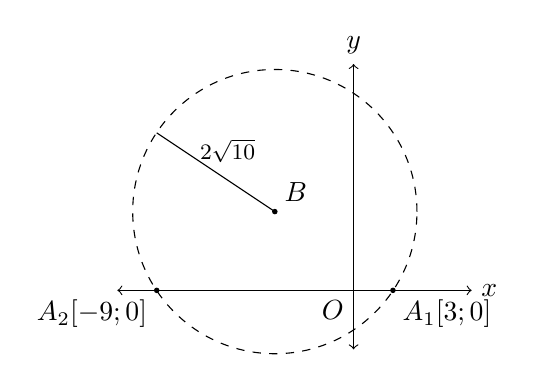
\begin{tikzpicture}[scale=0.5]
            \draw [<->] (-6,0) -- (3,0) node[right] {$x$};
            \draw [<->] (0,-1.5) -- (0,5.75) node[above] {$y$};
            \node[below left] at (0,0) {$O$};

            % Body
            \fill (-2,2) circle (2pt);
            \node[above right] at (-2,2) {$B$};

            \fill (1,0) circle (2pt);
            \node[below right] at (1,0) {$A_1[3;0]$};

            \fill (-5,0) circle (2pt);
            \node[below left] at (-5,0) {$A_2[-9;0]$};


            % Kruh se středem v bodě B a poloměrem AB
            \draw[dashed] (-2,2) circle (3.61); % Poloměr 2√10 ≈ 2.83
            \draw (-2,2) -- (-5,4);
            \node[above, font=\small] at (-3.2,3) {\footnotesize $2\sqrt{10}$};

        \end{tikzpicture}
        \caption{Znázornění bodů $A_1$, $A_2$ a $B$ v kartézské soustavě souřadnic}
        \label{fig:distance_example}
    \end{figure}

\end{example}



\subsubsection{Střed úsečky v rovině}\label{subsubsec:Midpoint_of_segment_in_plane}

Střed úsečky $AB$ je bod, který leží na úsečce $AB$ a je stejně vzdálen od obou koncových bodů $A$ a $B$.
Jinými slovy dělí úsečku $AB$ na dvě shodné části (viz Obrázek~\ref{fig:midpoint_of_segment}).

Nechť $A = [x_1; y_1]$ a $B = [x_2; y_2]$ jsou dva body v rovině.

\begin{definition}\label{def:midpoint}
    Střed $S$ úsečky $AB$ je bod daný vztahem
    \begin{equation}\label{eq:midpoint}
        S = \left[\frac{x_1 + x_2}{2}; \frac{y_1 + y_2}{2}\right].
    \end{equation}
\end{definition}

\begin{figure}[H]
    \centering
    \begin{tikzpicture}
        \draw [<->] (-1,0) -- (5,0) node[right] {$x$};
        \draw [<->] (0,-1) -- (0,5) node[above] {$y$};
        \node[below left] at (0,0) {$O$};

        % Body
        \fill (0.5,1) circle (2pt);
        \node[below left] at (0.5,1) {$A$};

        \fill (4,3) circle (2pt);
        \node[above right] at (4,3) {$B$};

        % Střed úsečky
        \fill (2.25,2) circle (2pt);
        \node[above right] at (2.25,2) {$S$};

        % Úsečka AB
        \draw[thick] (0.5,1) -- (4,3);

        % Kolmice k osám
        \draw[dashed] (0.5,1) -- (0.5,0);
        \draw[dashed] (4,3) -- (4,0);
        \node[below, font=\footnotesize] at (0.5,0) {$x_1$};
        \node[below, font=\footnotesize] at (4,0) {$x_2$};

        \draw[dashed] (0.5,1) -- (0,1);
        \draw[dashed] (4,3) -- (0,3);
        \node[left, font=\footnotesize] at (0,1) {$y_1$};
        \node[left, font=\footnotesize] at (0,3) {$y_2$};

        \draw[dashed] (2.25,2) -- (2.25,0);
        \node[below, font=\footnotesize] at (2.25,0) {$\frac{x_1 + x_2}{2}$};
        \draw[dashed] (2.25,2) -- (0,2);
        \node[left, font=\footnotesize] at (0,2) {$\frac{y_1 + y_2}{2}$};
        

    \end{tikzpicture}
    \caption{Střed úsečky $AB$ v kartézské soustavě souřadnic}
    \label{fig:midpoint_of_segment}
\end{figure}

\begin{remark}
    Souřadnice středu úsečky vzniknou jako \textbf{aritmetické průměry} souřadnic krajních bodů.
\end{remark}

\begin{example}
    Mějme body $A = [1;2]$ a $B = [9;-4]$.
    Střed úsečky $AB$ určíme pomocí vzorce~\eqref{eq:midpoint}:
    \[
    S = \left[\frac{1 + 9}{2}; \frac{2 + (-4)}{2}\right] = \left[\frac{10}{2}; \frac{-2}{2}\right] = \left[5; -1\right].
    \]
    Tedy střed úsečky $AB$ je bod $S$ s souřadnicemi $[5; -1]$.
\end{example}

\begin{example}
    Mějme bod $B = [9;-4]$ a střed úsečky $S = [5; -1]$.
    Chceme určit souřadnice druhého krajního bodu $A$ úsečky $AB$.
    Použijeme vzorec pro střed úsečky~\eqref{eq:midpoint} a dosadíme známé hodnoty:
    \[
    [5; -1] = \left[\frac{x_1 + 9}{2}; \frac{y_1 + (-4)}{2}\right].
    \]
    Z toho dostaneme dvě rovnice:
    \[
    5 = \frac{x_1 + 9}{2} \quad \Rightarrow \quad x_1 + 9 = 10 \quad \Rightarrow \quad x_1 = 1,
    \]
    \[
    -1 = \frac{y_1 - 4}{2} \quad \Rightarrow \quad y_1 - 4 = -2 \quad \Rightarrow \quad y_1 = 2.
    \]
    Tedy druhý krajní bod $A$ úsečky $AB$ má souřadnice $[1; 2]$.
\end{example}


\subsection{Body v prostoru}\label{subsec:Points_in_space}

Stejně jako jsme v rovině definovali body pomocí uspořádané dvojice reálných čísel $[x;y]$, v prostoru budeme definovat body pomocí uspořádané trojice reálných čísel $[x;y;z]$.


\begin{definition}\label{def:bod_v_prostoru}
    Bodem v prostoru rozumíme uspořádanou trojici reálných čísel
    \[
    A = [x;y;z], \quad x,y,z \in \mathbb{R}.
    \]
    Číslo $x$ nazýváme první souřadnicí, číslo $y$ druhou souřadnicí a číslo $z$ třetí souřadnicí.
\end{definition}

\begin{example}
    Mějme body $A = [-2,2,3]$ a $B = [4,3,-2]$, které chceme zakreslit do kartézské soustavy souřadnic v prostoru (viz Obrázek~\ref{fig:cartesian_space_points}).
    Tyto body se nacházejí v různých oktantech prostoru:
    \begin{figure}[H]
        \centering
        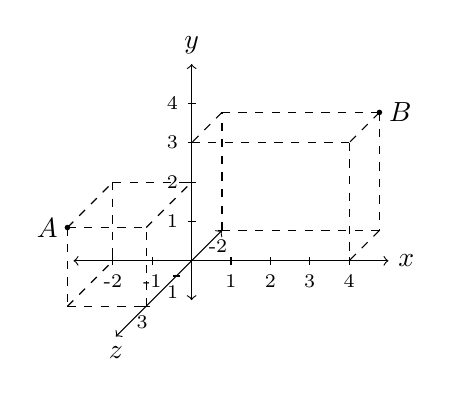
\begin{tikzpicture}[scale=0.5]
            \draw [<->] (-3,0) -- (5,0) node[right] {$x$};
            \draw [<->] (0,-1) -- (0,5) node[above] {$y$};
            \draw [<->] (0,0,-2) -- (0,0,5) node[below] {$z$};

            \foreach \x in {-2,-1,1,2,3,4} {
                \draw (\x,0.1,0) -- (\x,-0.1,0) node[below, font=\scriptsize] {\x};
            }

            \foreach \y in {1,2,3,4} {
                \draw (0.1,\y,0) -- (-0.1,\y,0) node[left, font=\scriptsize] {\y};
            }

            \foreach \z in {-2,1,3} {
                \draw (0.1,0,\z) -- (-0.1,0,\z) node[below, font=\scriptsize] {\z};
            }

            % Body
            \fill (-2,2,3) circle (2pt);
            \node[left] at (-2,2,3) {$A$};

            \fill (4,3,-2) circle (2pt);
            \node[right] at (4,3,-2) {$B$};

            % Pomocné čáry pro lepší orientaci
            % Bod A
            \draw[dashed] (-2,2,0) -- (-2,0,0);
            \draw[dashed] (-2,2,3) -- (-2,2,0);
            \draw[dashed] (-2,2,3) -- (-2,0,3);
            \draw[dashed] (-2,2,3) -- (0,2,3);
            \draw[dashed] (-2,2,0) -- (0,2,0);
            \draw[dashed] (-2,0,3) -- (0,0,3);
            \draw[dashed] (-0,0,3) -- (0,2,3);
            \draw[dashed] (0,2,3) -- (0,2,0);
            \draw[dashed] (-2,0,3) -- (-2,0,0);
            % Bod B
            \draw[dashed] (4,3,-2) -- (4,3,0);
            \draw[dashed] (4,3,-2) -- (4,0,-2);
            \draw[dashed] (4,3,-2) -- (0,3,-2);
            \draw[dashed] (4,3,0) -- (0,3,0);
            \draw[dashed] (4,0,-2) -- (0,0,-2);
            \draw[dashed] (0,3,-2) -- (0,3,0);
            \draw[dashed] (4,3,0) -- (4,0,0);
            \draw[dashed] (4,0,-2) -- (4,0,0);
            \draw[dashed] (0,0,-2) -- (0,3,-2);
        \end{tikzpicture}
        \caption{Znázornění bodů v kartézské soustavě souřadnic v prostoru}
        \label{fig:cartesian_space_points}
\end{figure}

\end{example}


\subsubsection{Vzdálenost dvou bodů v prostoru}\label{subsubsec:Distance_between_points_in_space}
Analogicky jako v rovině lze určit vzdálenost dvou bodů i v prostoru, ale místo dvou souřadnic $[x;y]$ budeme mít tři souřadnice $[x;y;z]$ a vzorec pro vzdálenost bude obsahovat další člen pro třetí rozměr.
\begin{definition}\label{def:distance_in_space}
    Nechť $A = [x_1; y_1; z_1]$ a $B = [x_2; y_2; z_2]$ jsou dva body v prostoru.
    Vzdálenost těchto bodů, označovaná $d = |AB|$, je dána vztahem
    \begin{equation}\label{eq:distance_in_space}
        d = \sqrt{(x_2 - x_1)^2 + (y_2 - y_1)^2 + (z_2 - z_1)^2}.
    \end{equation}
\end{definition}

\begin{example}
    Mějme body $A = [0;-1;3]$ a $B = [-4,1,-1]$.
    Vzdálenost mezi těmito body určíme pomocí vzorce~\eqref{eq:distance_in_space}:
    \[
    d = \sqrt{(-4 - 0)^2 + (1 - (-1))^2 + (-1 - 3)^2} = \sqrt{(-4)^2 + 2^2 + (-4)^2}  = \sqrt{36} = 6.
    \]
    Tedy vzdálenost mezi body $A$ a $B$ je $6$ jednotek.
\end{example}


\subsubsection{Střed úsečky v prostoru}\label{subsubsec:Midpoint_of_segment_in_space}
Analogicky jako v rovině lze určit střed úsečky i v prostoru, ale místo dvou souřadnic $[x;y]$ budeme mít tři souřadnice $[x;y;z]$ a vzorec pro střed úsečky bude obsahovat další člen pro třetí rozměr.
\begin{definition}\label{def:midpoint_in_space}
    Nechť $A = [x_1; y_1; z_1]$ a $B = [x_2; y_2; z_2]$ jsou dva body v prostoru.
    Střed $S$ úsečky $AB$ je bod daný vztahem
    \begin{equation}\label{eq:midpoint_in_space}
        S = \left[\frac{x_1 + x_2}{2}; \frac{y_1 + y_2}{2}; \frac{z_1 + z_2}{2}\right].
    \end{equation}
\end{definition}

\begin{example}
    Mějme body $A = [2;1;-3]$ a $B = [2;-3;3]$.
    Střed úsečky $AB$ určíme pomocí vzorce~\eqref{eq:midpoint_in_space}:
    \[
    S = \left[\frac{2 + 2}{2}; \frac{1 + (-3)}{2}; \frac{-3 + 3}{2}\right] = \left[2; -1; 0\right].
    \]
    Tedy střed úsečky $AB$ je bod $S$ s souřadnicemi $[2; -1; 0]$.
\end{example}

\begin{example}
    Mějme bod $B = [2;-3;3]$ a střed úsečky $S = [2; -1; 0]$.
    Chceme určit souřadnice druhého krajního bodu $A$ úsečky $AB$.
    Použijeme vzorec pro střed úsečky~\eqref{eq:midpoint_in_space} a dosadíme známé hodnoty:
    \[
    [2; -1; 0] = \left[\frac{x_1 + 2}{2}; \frac{y_1 + (-3)}{2}; \frac{z_1 + 3}{2}\right].
    \]
    Z toho dostaneme tři rovnice:
    \[
    2 = \frac{x_1 + 2}{2} \quad \Rightarrow \quad x_1 + 2 = 4 \quad \Rightarrow \quad x_1 = 2,
    \]
    \[
    -1 = \frac{y_1 - 3}{2} \quad \Rightarrow \quad y_1 - 3 = -2 \quad \Rightarrow \quad y_1 = 1,
    \]
    \[
    0 = \frac{z_1 + 3}{2} \quad \Rightarrow \quad z_1 + 3 = 0 \quad \Rightarrow \quad z_1 = -3.
    \]
    Tedy druhý krajní bod $A$ úsečky $AB$ má souřadnice $[2; 1; -3]$.
\end{example}





